\section{Jak dlouhé je pobřeží Velké Británie?}\label{sec:pobrezi_velke_britanie}
Položme si na začátek trochu jinou otázku,~kterou si z~počátku položil i~Benoît Mandelbrot: \emph{Jaká je podstata tvaru pobřeží?} Ta se stala podstatnou v~jeho práci \emph{"How Long Is the Coast of Britain?"}. Uvažme část pobřeží s~počátečním a~koncovým bodem (viz obrázek~\ref{fig:pobrezi}).
\begin{figure}[h]
    \centering
    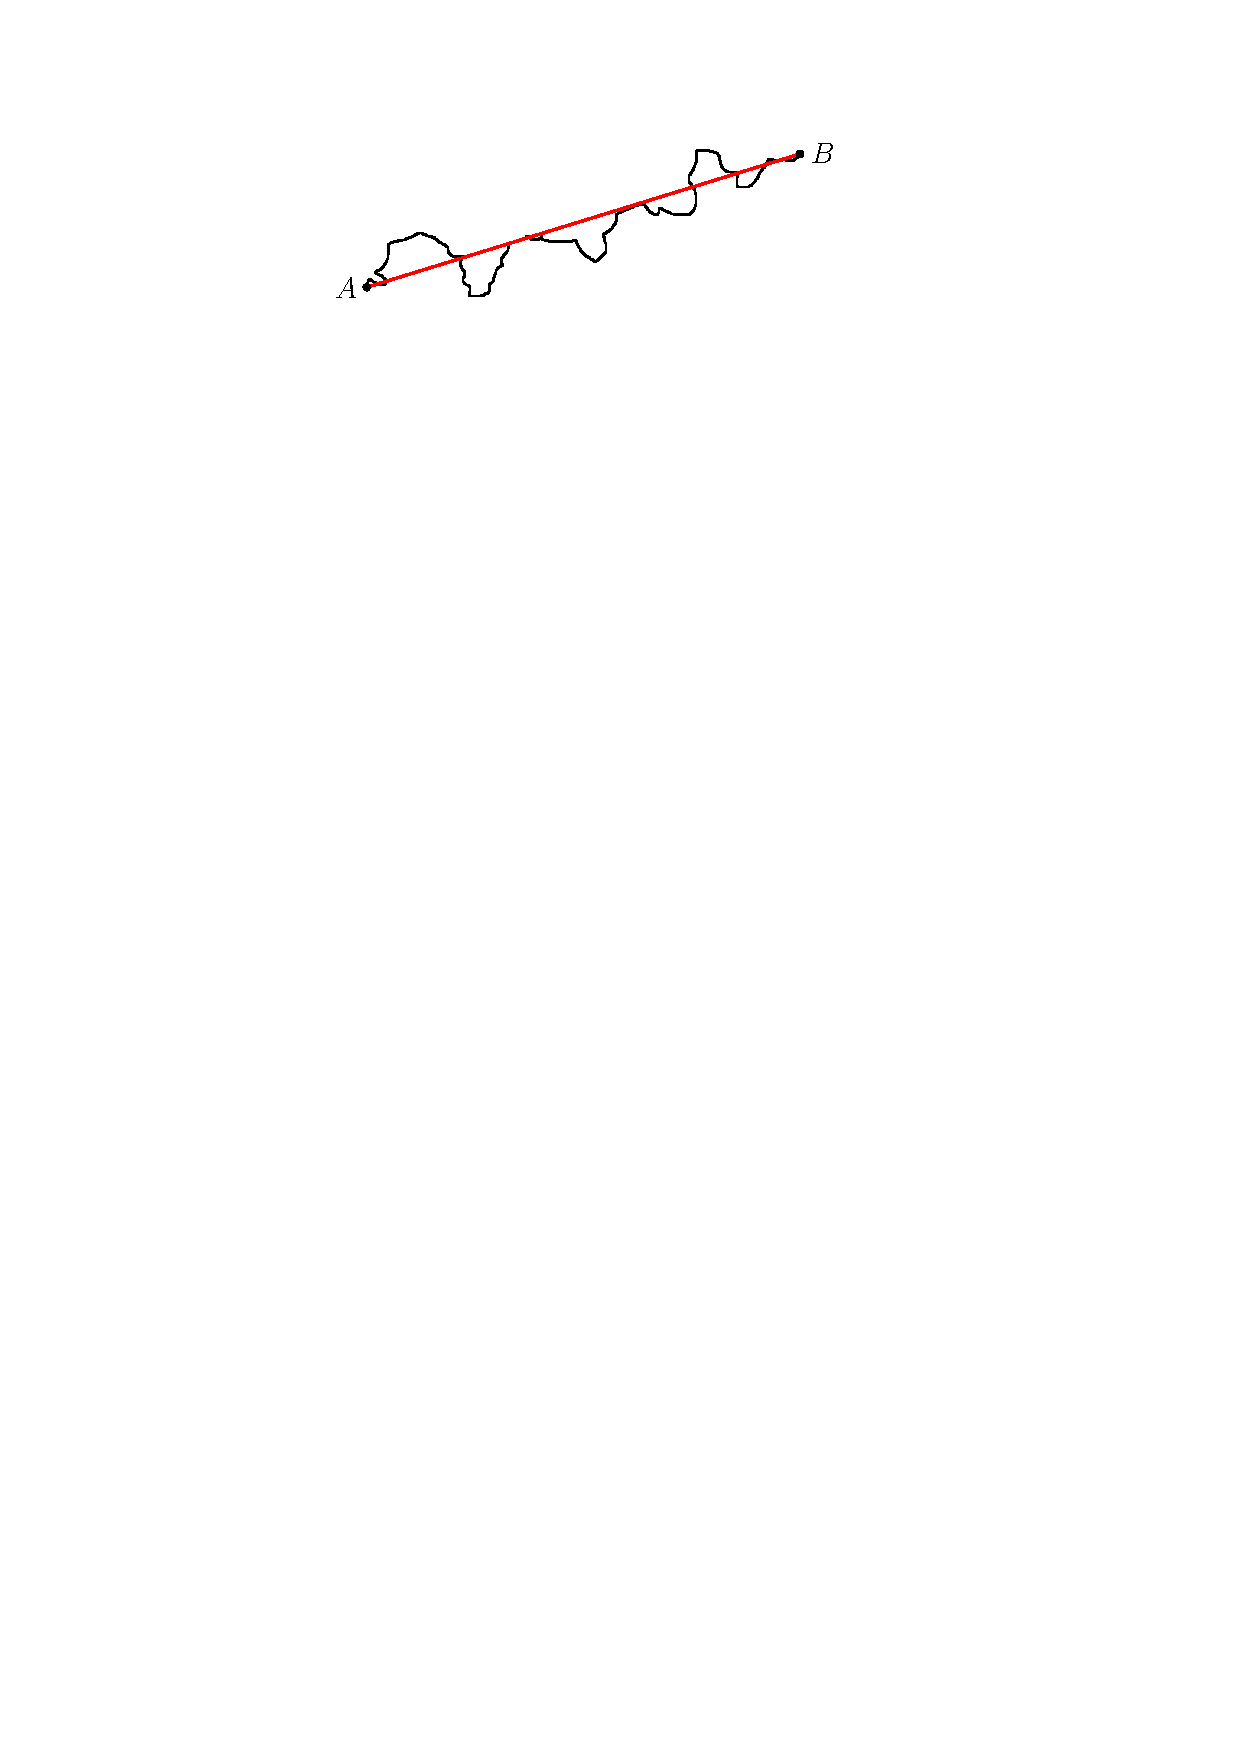
\includegraphics[scale=\normalipe]{ch01-pobrezi.pdf}
    \caption{Příklad mapy pobřeží se spojnicí bodů $A$ a~$B$.}
    \label{fig:pobrezi}
\end{figure}
Zjevně jeho délka je zdola omezena délkou spojnice koncových bodů $A$ a~$B$,~nicméně typické pobřeží je velmi nepravidelné a~klikaté. Existují různé metody,~které nám umožňují určit jeho délku přesněji. Několik z~nich je popsáno v~knize \citep[str. 79]{Mandelbrot1983},~pro uvedení do problematiky si zde však vystačíme s~tou nejednodušší.\par
Předpokládejme,~že pobřeží,~které zkoumáme,~má pevné hranice (tj. zanedbáváme např. přílivy a~odlivy nastávající během dne),~a dále jsme schopni rozlišovat libovolně krátké vzdálenosti.\par
Mějme zadané libovolné $\varepsilon>0$. Podél pobřeží začneme umisťovat tyče tak,~že po každém umístění provedeme na mapě krok délky \textbf{nejvýše} $\varepsilon$,~přičemž začínáme v~bodě $A$ a~postupujeme až k~bodu $B$ (popř. pokud měříme délku pobřeží ostrova,~pokračujeme dokud se nevrátíme tam,~kde jsme začali). Předpokládejme,~že jsme provedli celkově $n(\varepsilon)$ kroků (jejich počet je závislý na zvolené délce kroku). \emph{Přibližnou délku pobřeží} $\ell(\varepsilon)$ pak stanovíme jako
\begin{equation*}
    \ell(\varepsilon)=n(\varepsilon)\cdot\varepsilon.
\end{equation*}
\begin{figure}[h]
    \centering
    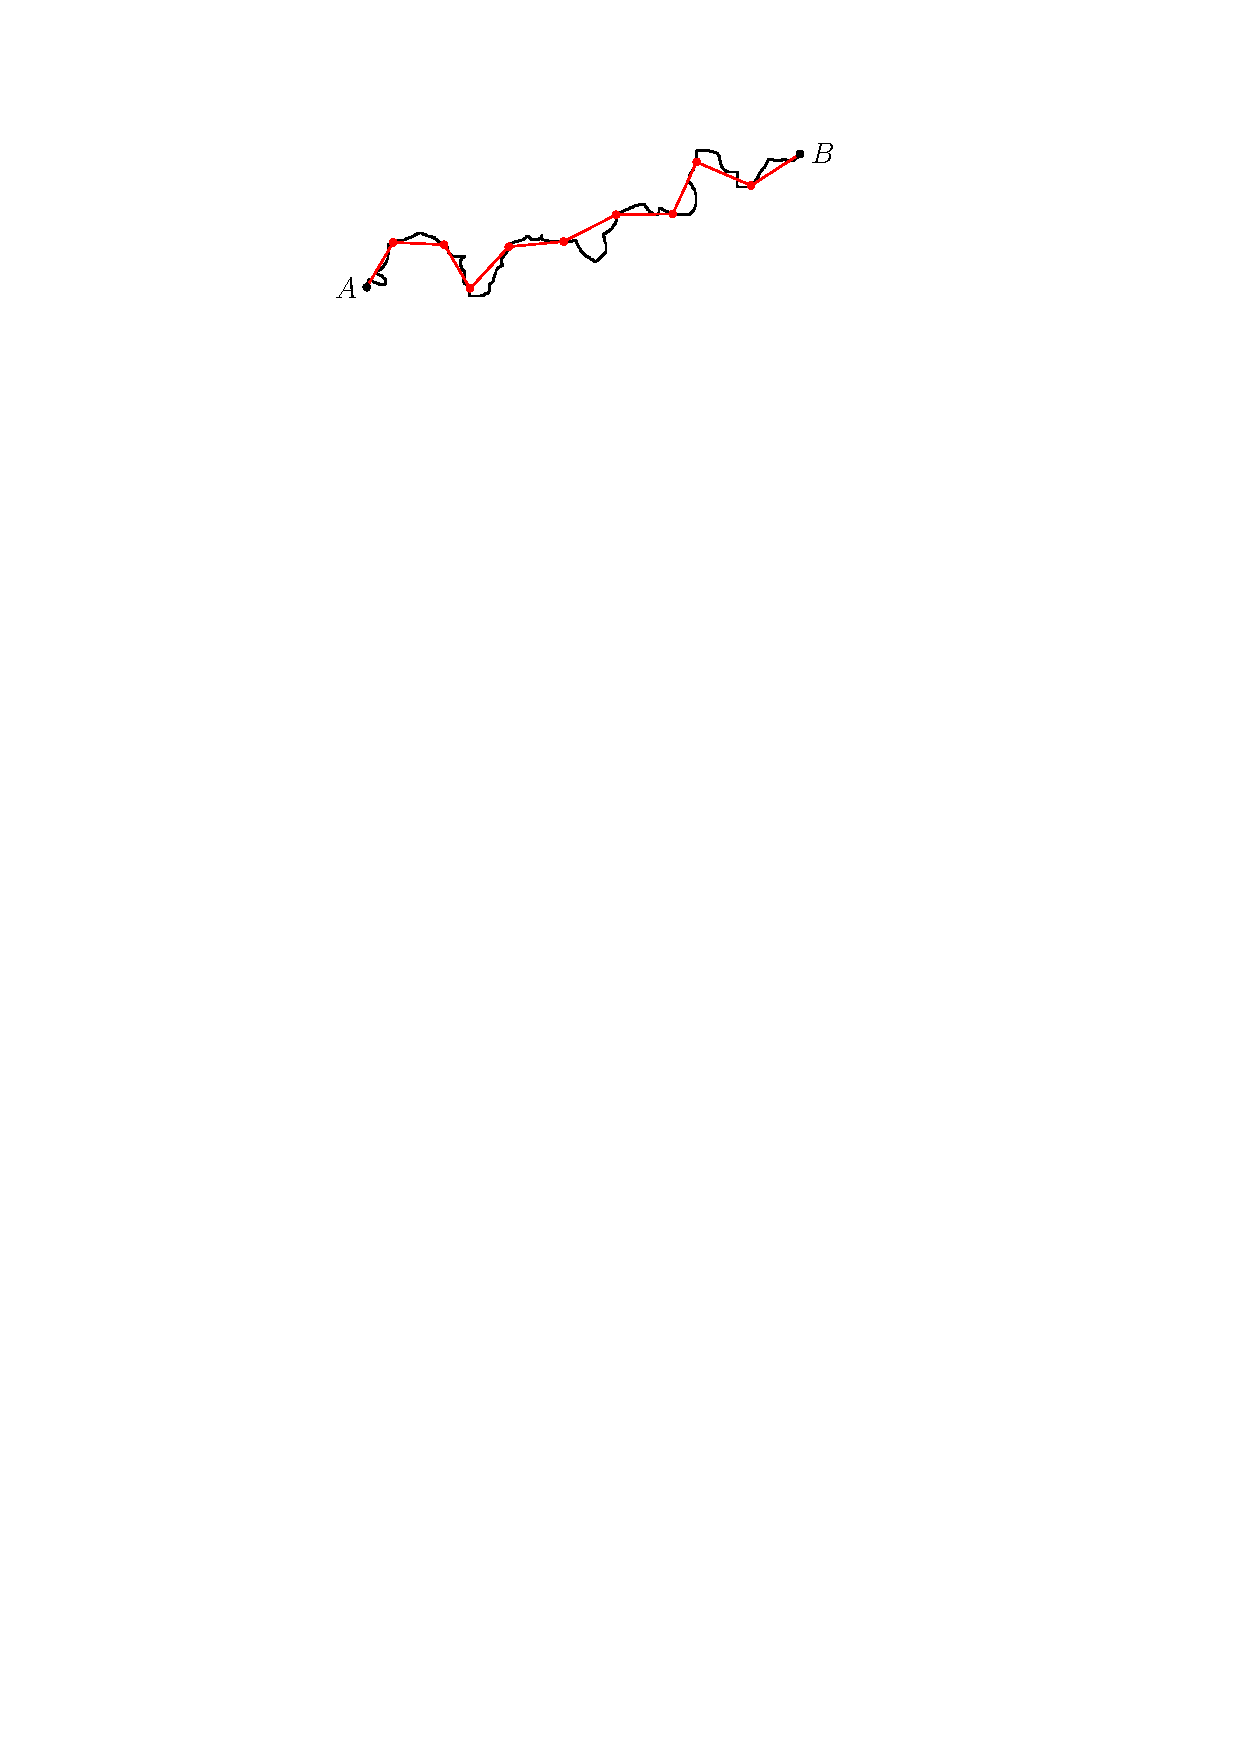
\includegraphics[scale=\normalipe]{ch01-pobrezi-aproximace.pdf}
    \caption{Odhad délky pobřeží,~kde $n=10$ při zvoleném $\varepsilon$.}
    \label{fig:pobrezi_aproximace}
\end{figure}
Nyní by nás mohlo napadnout,~že pro zmenšující se $\varepsilon$,~tj. $\varepsilon\to0_+$,~bude hodnota $\ell(\varepsilon)$ konvergovat ke skutečné délce pobřeží. Tzn.~označíme-li skutečnou délku pobřeží $L$,~pak bychom mohli očekávat,~že platí
\begin{equation}\label{eq:aproximace_limita}
    L=\lim_{\varepsilon\to0_+}{\ell(\varepsilon)}.
\end{equation}
Jenže,~bohužel,~limita \eqref{eq:aproximace_limita} bude v reálné situaci rovna $\infty$. Proč? Je třeba si uvědomit,~že zde pracujeme s~\emph{mapou} pobřeží,~která má určité \emph{měřítko}. Pokud bychom měli pobřeží na mapě s~měřítkem $1\,:\,100\;000$,~uvidíme méně detailů,~než kdybychom jej zkoumali na mapě s~měřítkem $1\,:\,1\;000$. (Viz obrázek~\ref{fig:pobrezi_zoom}.)\par
\begin{figure}[h]
    \centering
    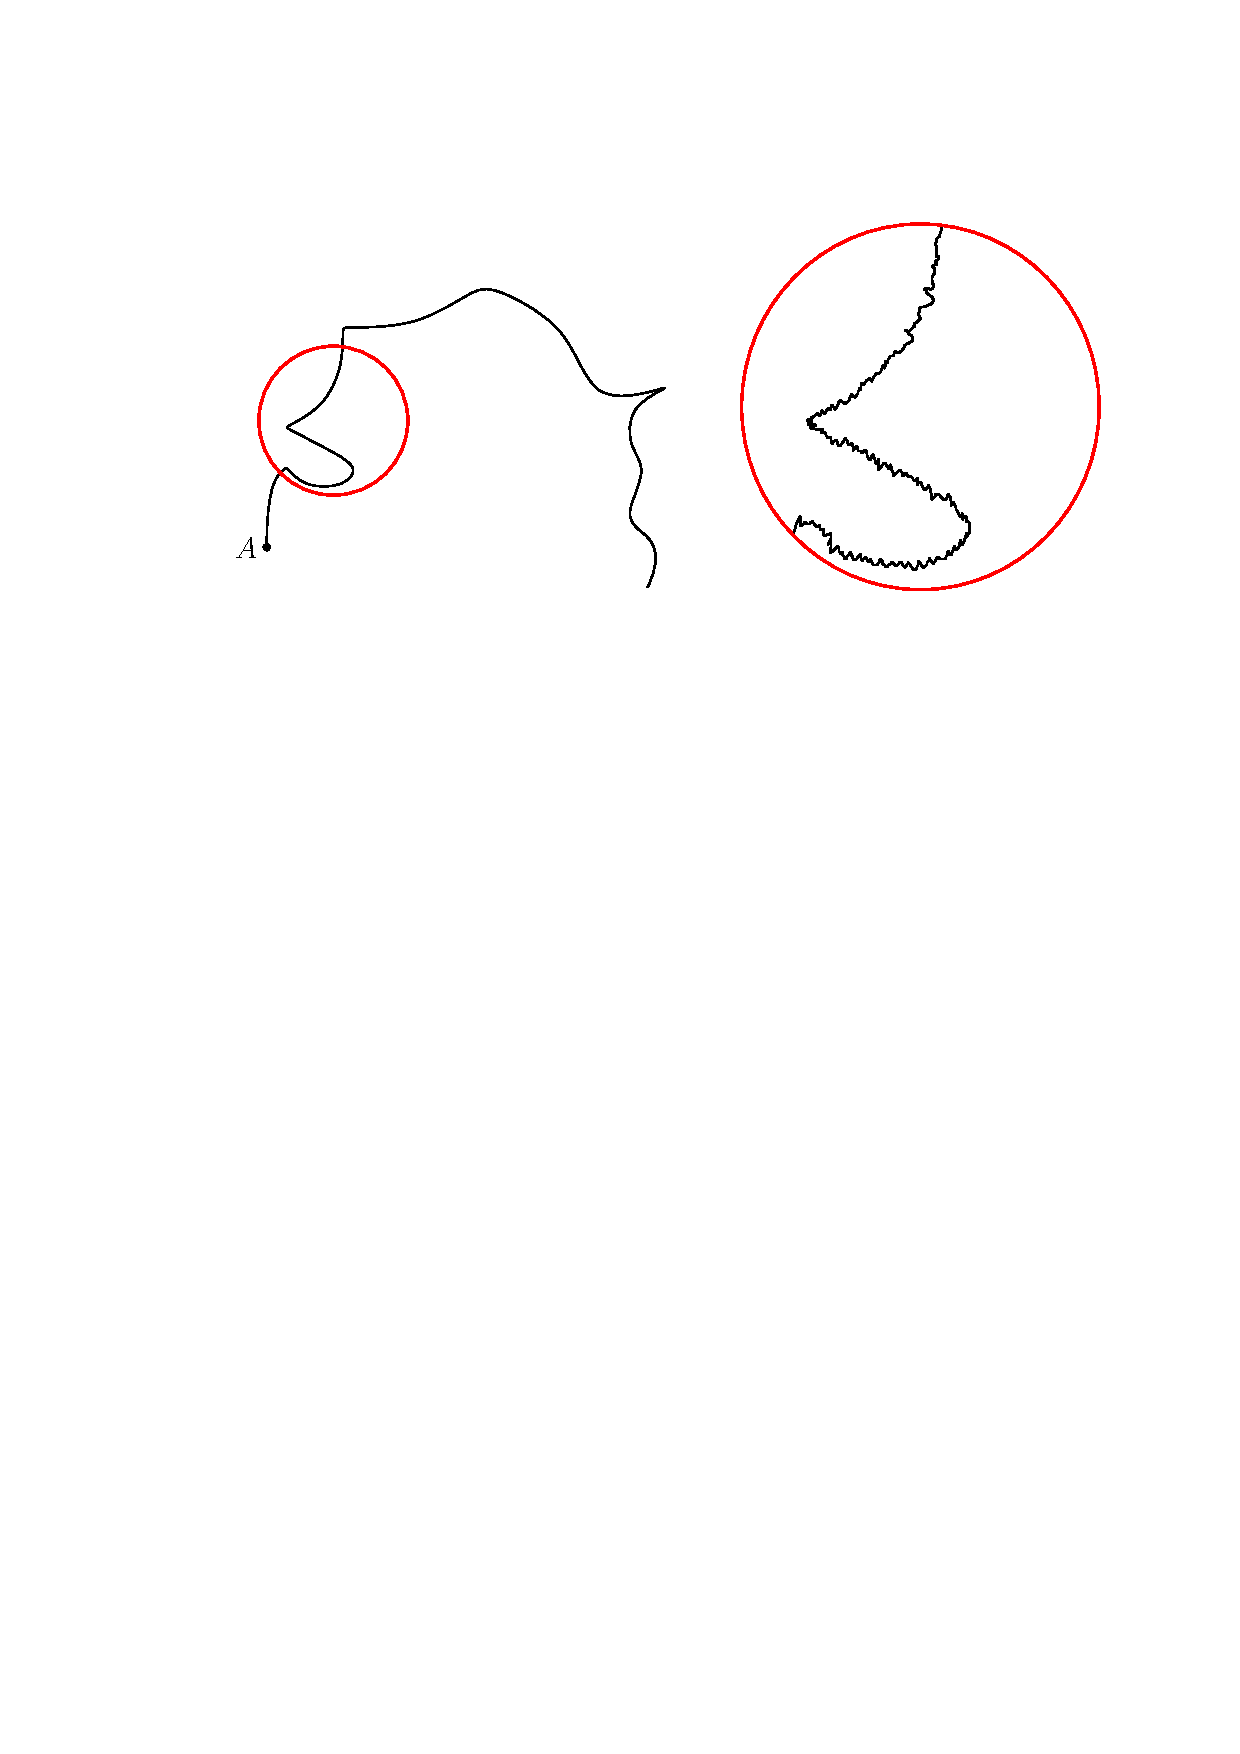
\includegraphics[scale=\normalipe]{ch01-pobrezi-zoom.pdf}
    \caption{Část pobřeží od bodu $A$ v~menším měřítku.}
    \label{fig:pobrezi_zoom}
\end{figure}
Nově odhalené detaily (menší poloostrůvky apod.) zde přispívají k~celkové délce pobřeží $\ell(\varepsilon)$. Postupným zvětšováním měřítka mapy bychom tak odhalili další detaily. Naše původní idea tak selhává,~neboť (v "klasickém" pojetí délky) pro $\varepsilon\to0_+$ hodnota $\ell(\varepsilon)$ patrně poroste nade všechny meze,~tj. $\lim_{\varepsilon\to0_+}{\ell(\varepsilon)}=\infty$.\par
Nabízí se otázka: Proč se toto děje? Pokud se ohlédneme zpět za eukleidovskou geometrií\index{geometrie!eukleidovská}\index{eukleidovská geometrie},~tento problém v ní nenastává. Např. u~kružnice v~eukleidovské rovině $\mathbb{E}_2$ změnou měřítka žádné další detaily křivky neobjevíme (podobně u~jiných geometrických útvarů,~viz obrázky~\ref{subfig:kruznice} a~\ref{subfig:kruznice_zoom}). 
\begin{figure}[h]
    \centering
    \begin{subfigure}{\subfigwidth}
        \centering
        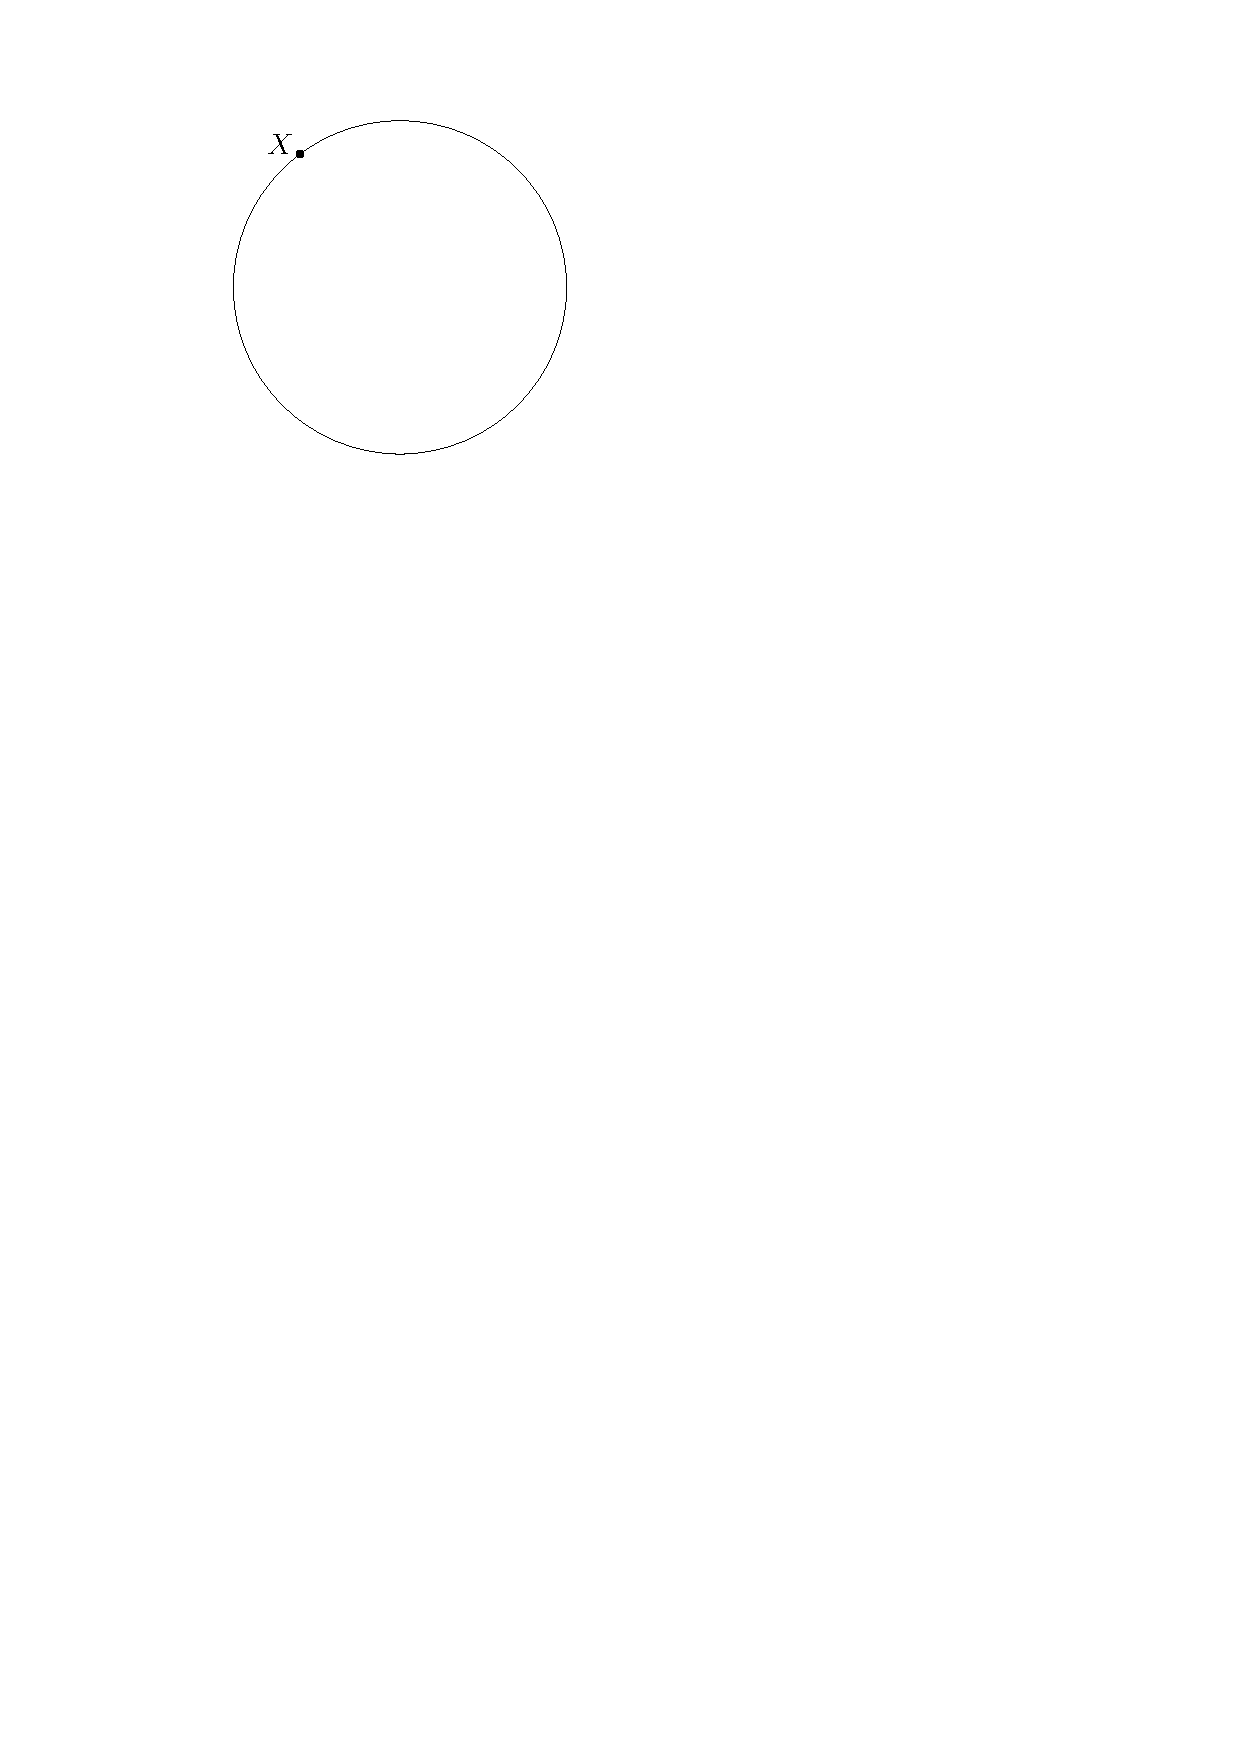
\includegraphics[scale=\normalipe]{ch01-kruznice.pdf}
        \caption{Kružnice v~menším měřítku.}
        \label{subfig:kruznice}
    \end{subfigure}
    \quad
    \begin{subfigure}{\subfigwidth}
        \centering
        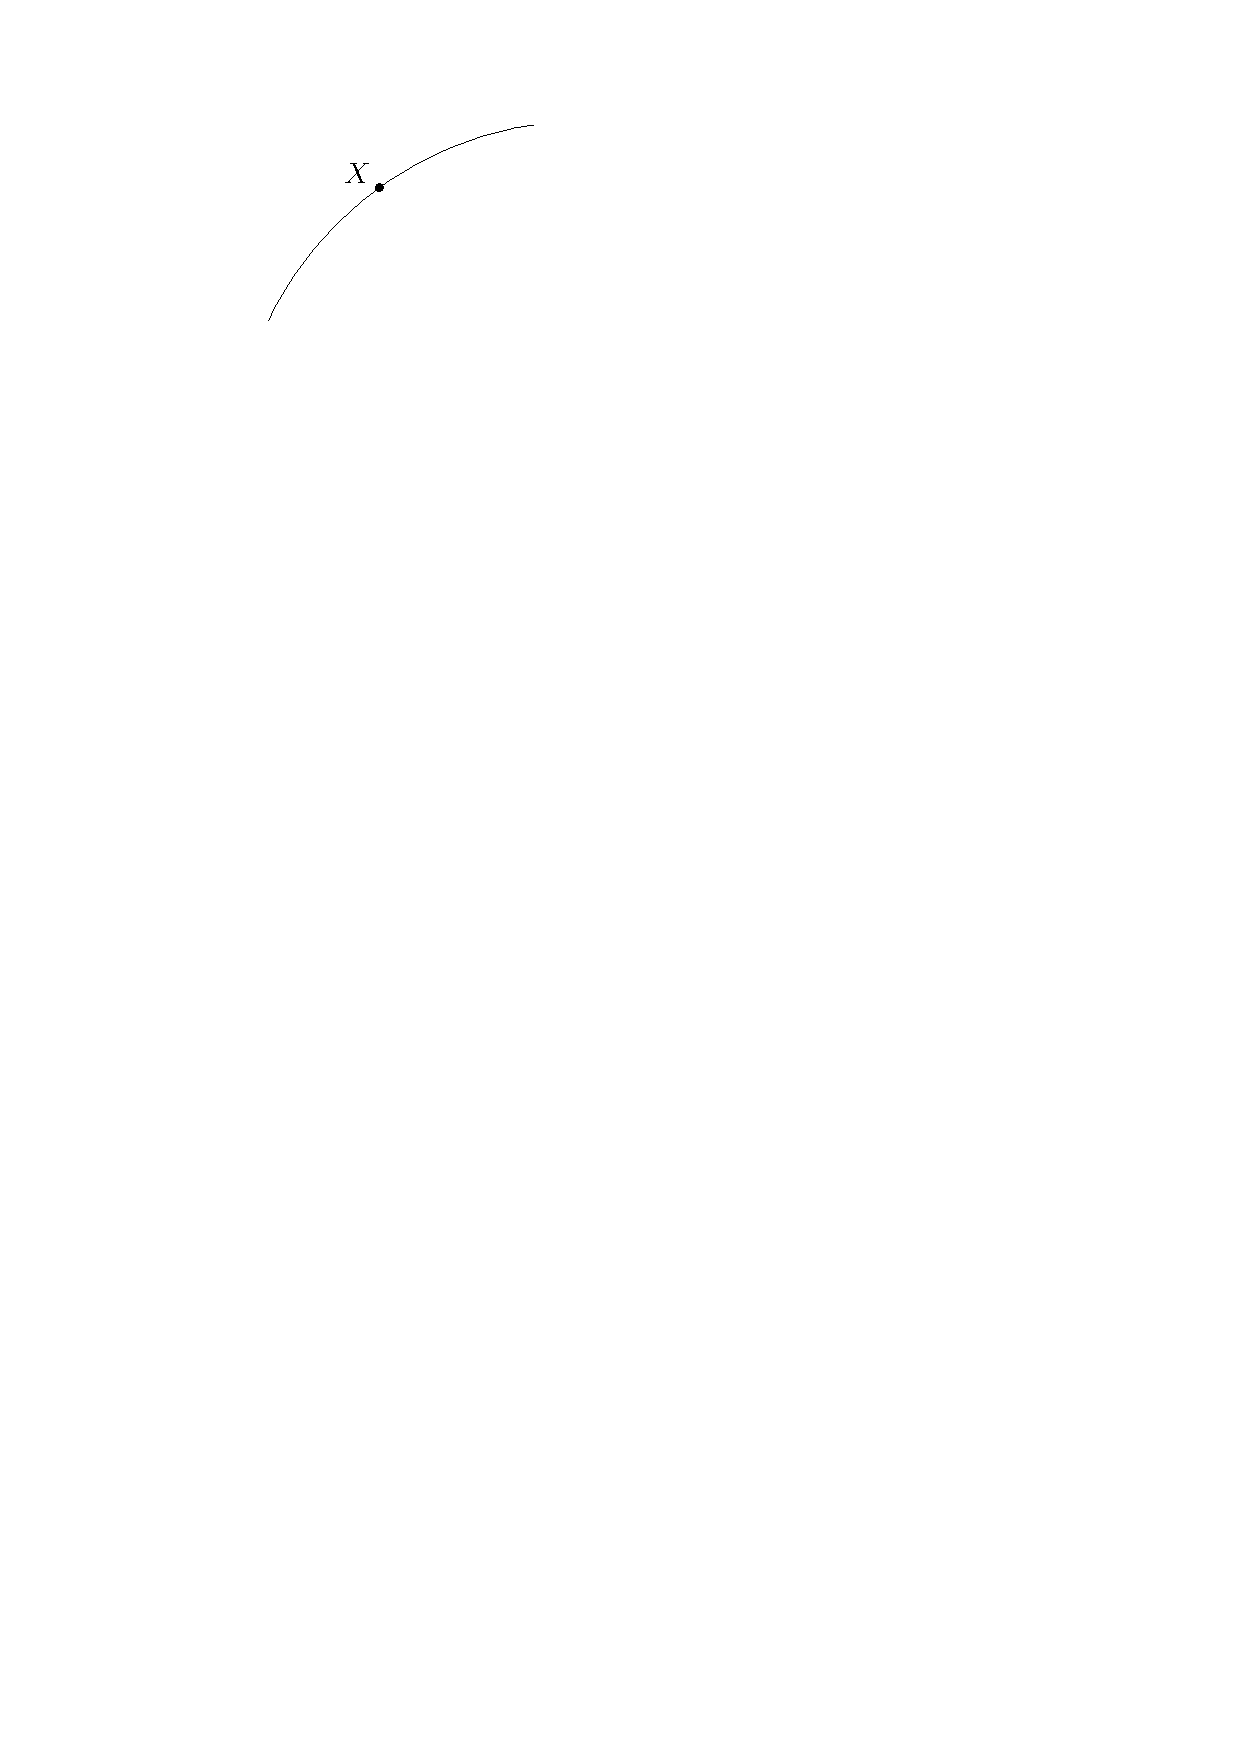
\includegraphics[scale=\normalipe]{ch01-kruznice-zoom.pdf}
        \caption{Část kružnice ve větším měřítku.}
        \label{subfig:kruznice_zoom}
    \end{subfigure}
\end{figure}
Díky tomu můžeme v~případě počítání obvodu kružnice použít následující postup.\par
Máme-li kružnici o~poloměru $r>0$,~pak jí můžeme vepsat libovolný pravidelný $n$-úhelník (viz obrázek~\ref{subfig:archimedova_metoda}).
\begin{figure}[h]
    \centering
    \begin{subfigure}{\subfigwidth}
        \centering
        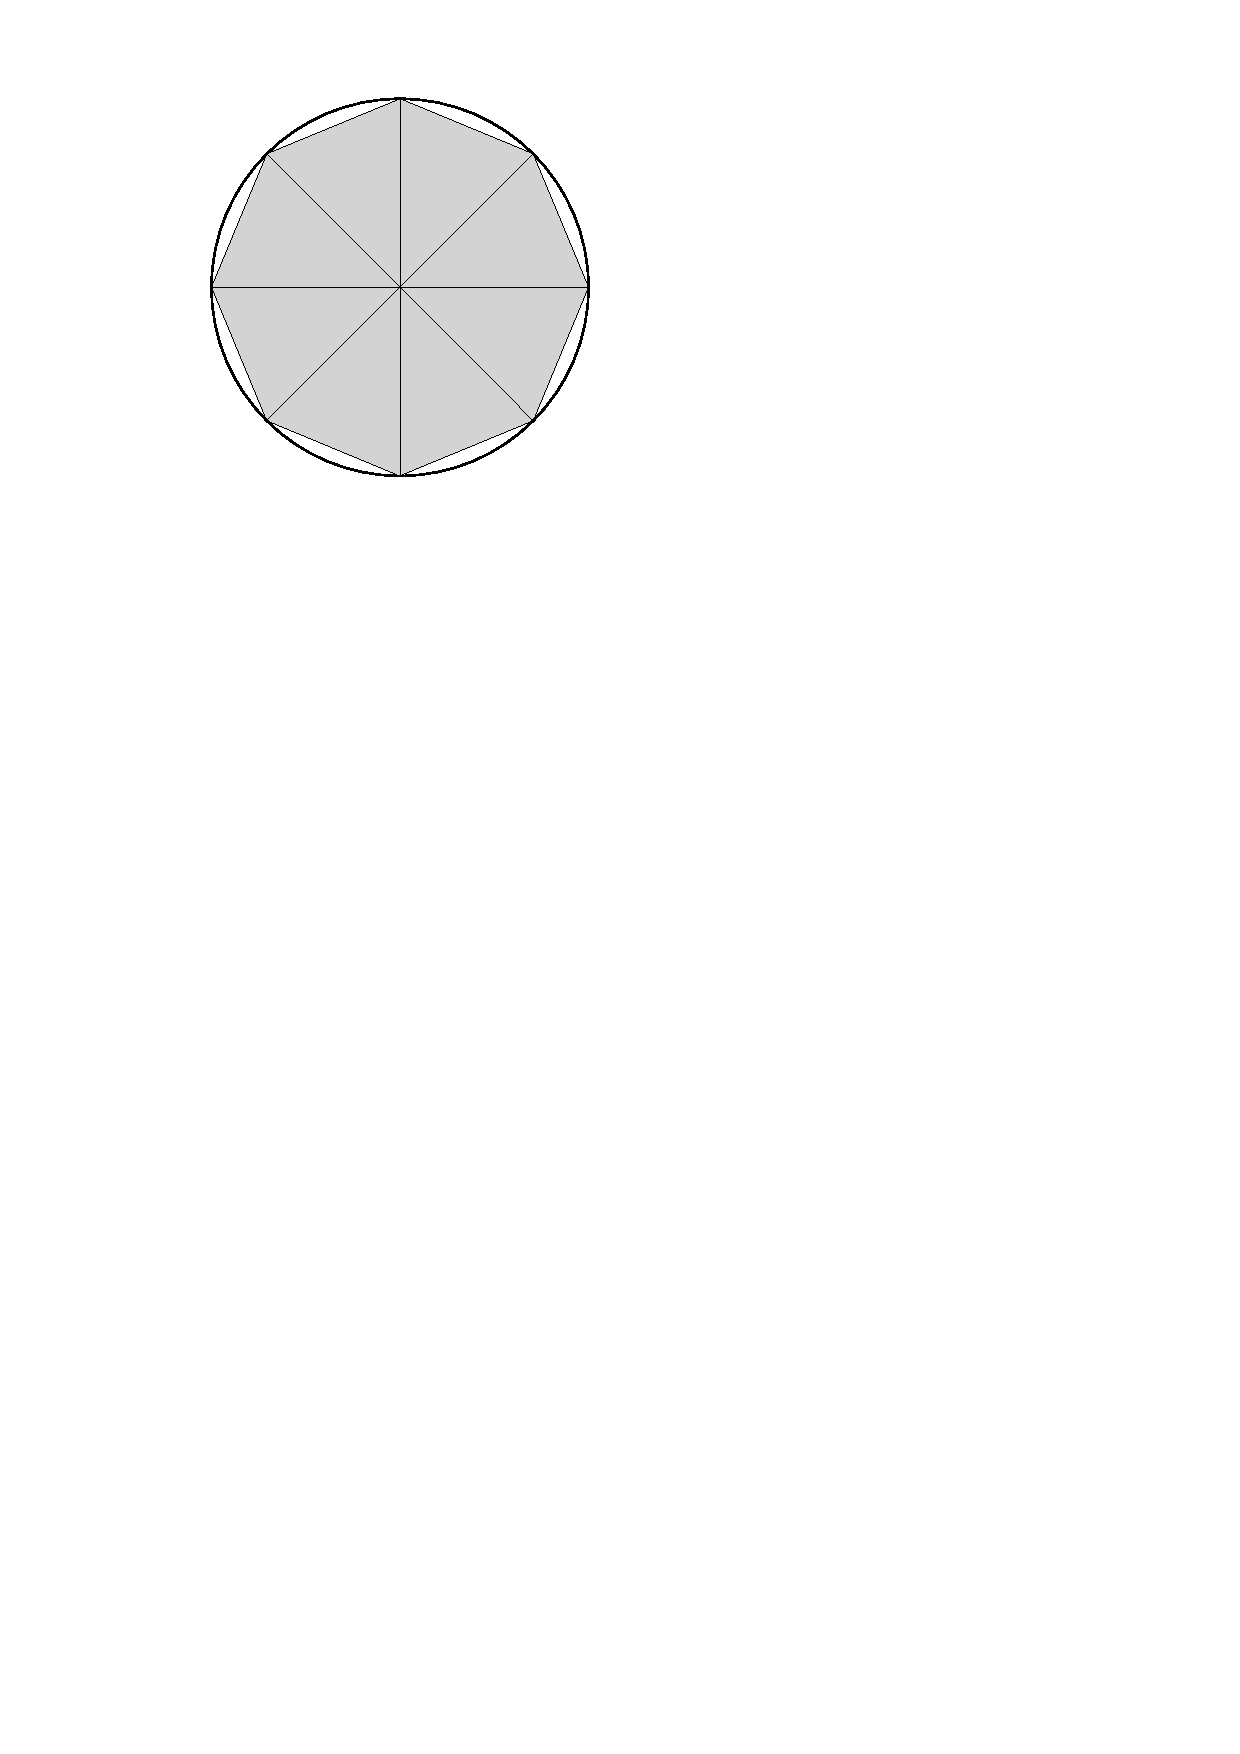
\includegraphics[scale=\normalipe]{ch01-archimedova-metoda.pdf}
        \caption{Pravidelný osmiúhelník vepsaný kružnici.}
        \label{subfig:archimedova_metoda}
    \end{subfigure}
    \quad
    \begin{subfigure}{\subfigwidth}
        \centering
        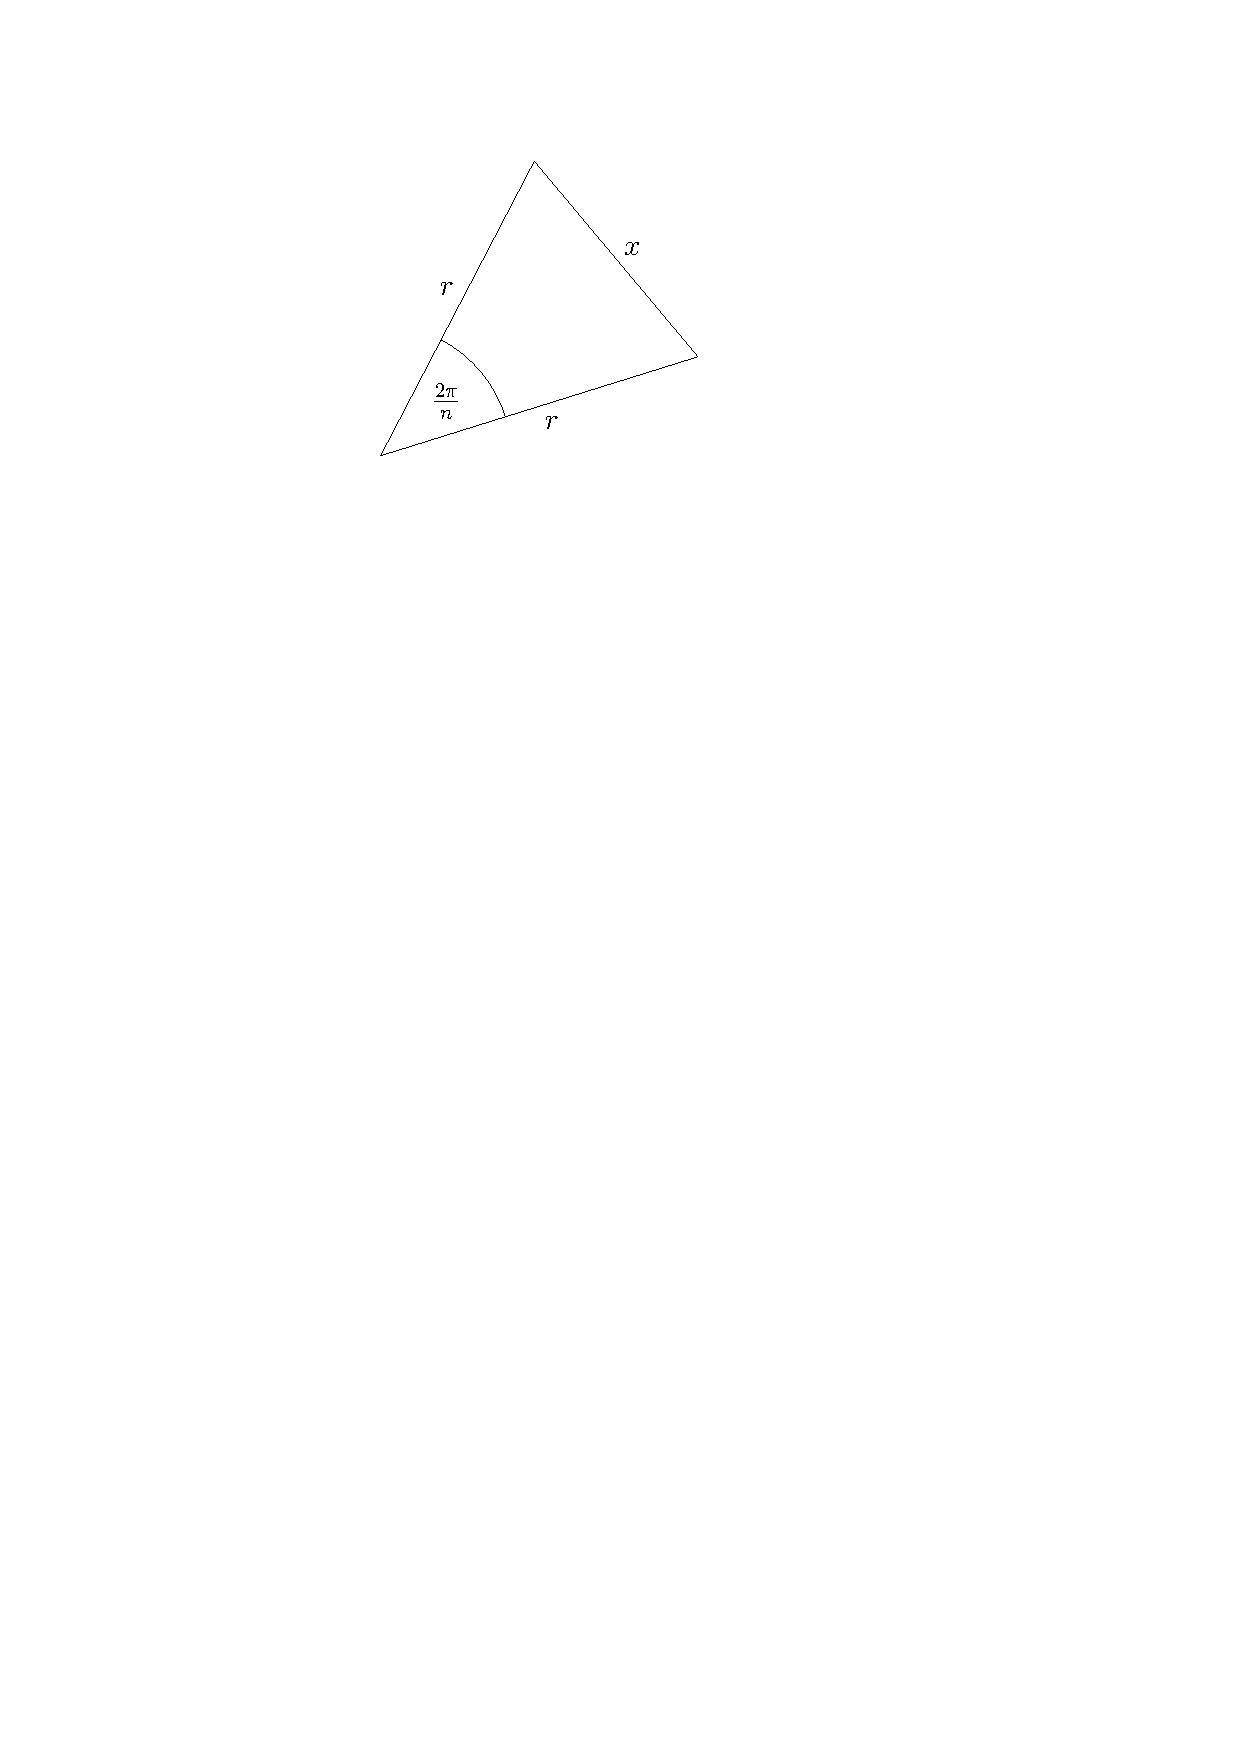
\includegraphics[scale=\normalipe]{ch01-archimedova-metoda-cast-nuhelniku.pdf}
        \caption{Část vepsaného pravidelného $n$-úhelníku.}
        \label{subfig:archimedova_metoda_cast_nuhelniku}
    \end{subfigure}
    \caption{Princip Archimédovy metody.}
    \label{fig:princip_archimedovy_metody}
\end{figure}
Obvod pravidelného $n$-úhelníku is označíme $O_n$ a~délku jeho strany $x$ (viz obrázek~\ref{subfig:archimedova_metoda_cast_nuhelniku}). Tu jsme schopni stanovit užitím elementární goniometrie,~tj.
\begin{equation*}
    x=2r\cdot\sin{\dfrac{\pi}{n}},
\end{equation*}
a tedy obvod
\begin{equation*}
    O_n=2rn\cdot\sin{\dfrac{\pi}{n}}.
\end{equation*}
Pro rostoucí $n$ bude obvod pravidelného $n$-úhelníku stále lépe aproximovat obvod původní kružnice (viz obrázek~\ref{fig:archimedova_metoda_presnejsi}).
\begin{figure}[h]
    \centering
    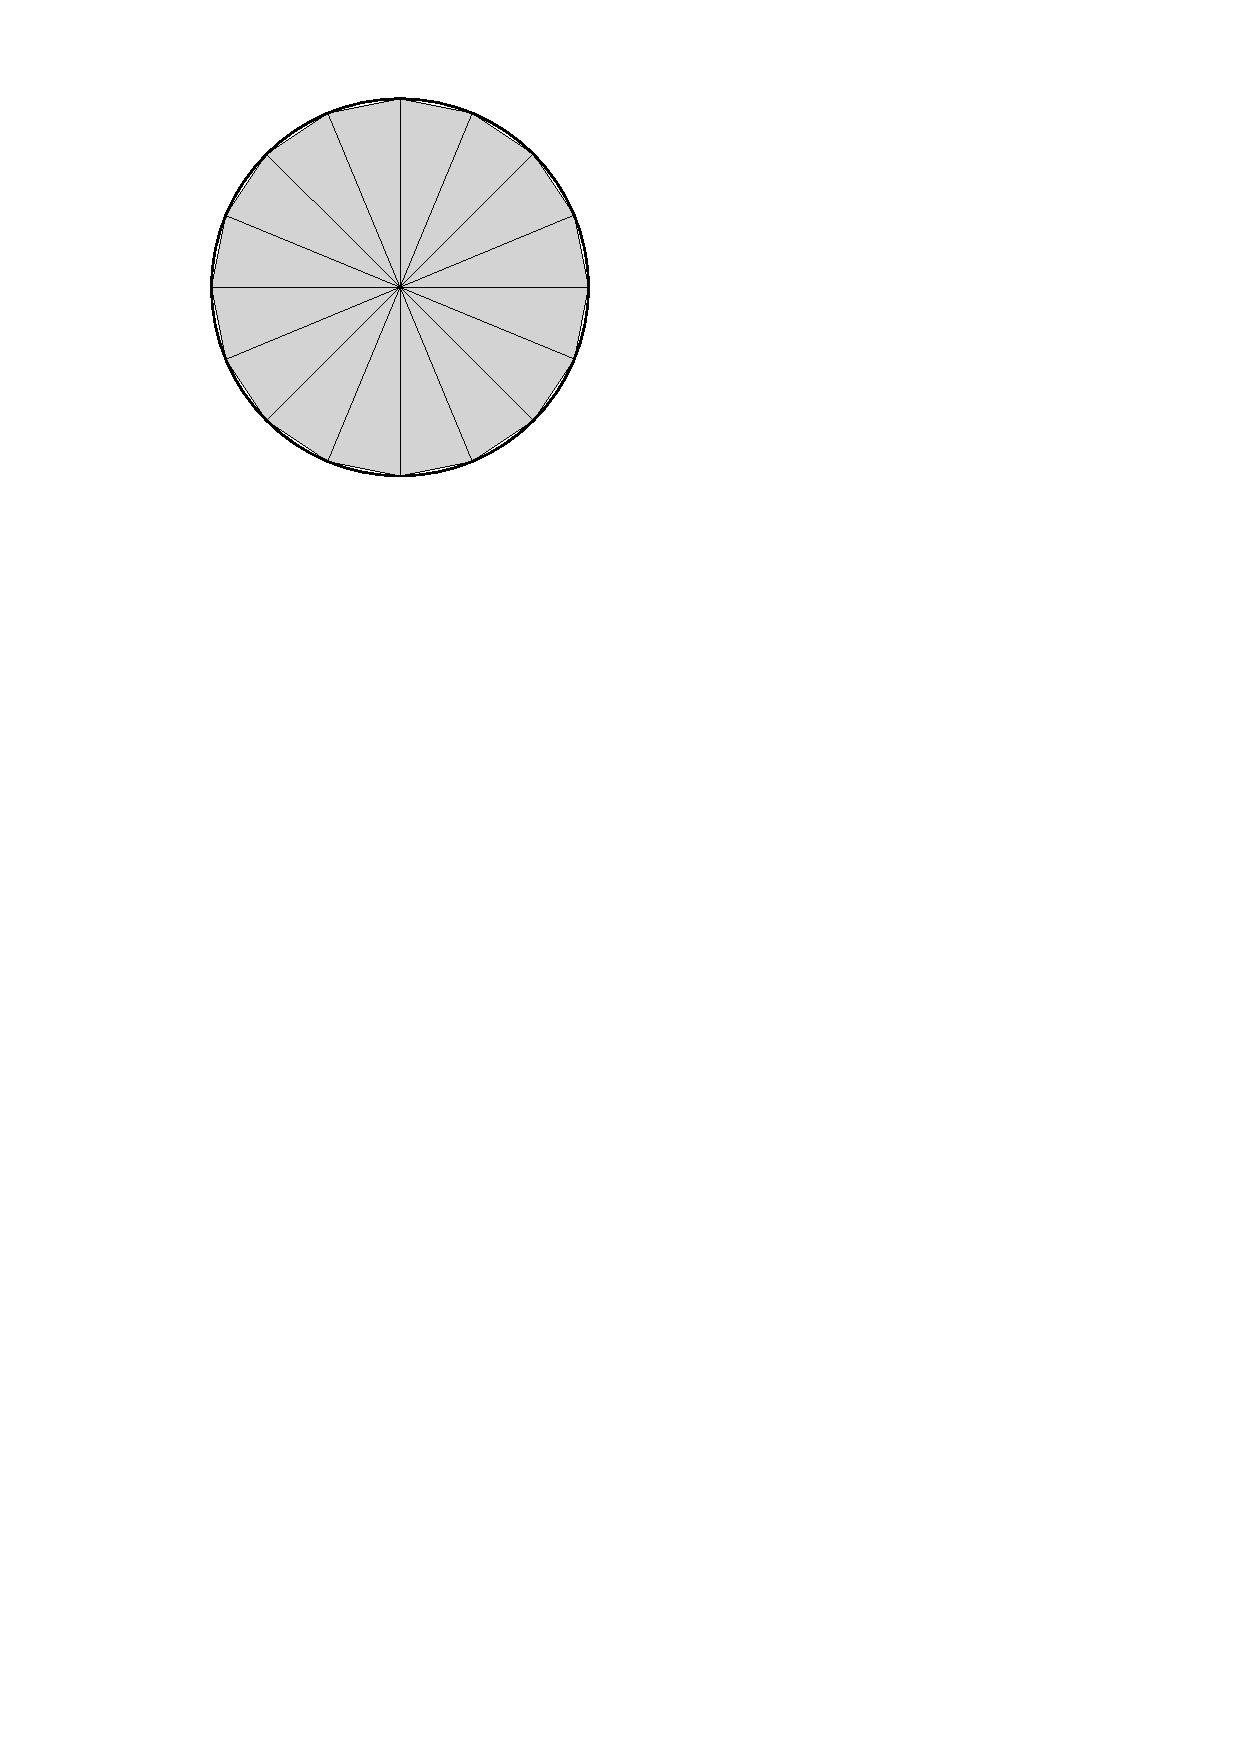
\includegraphics[scale=\normalipe]{ch01-pobrezi-aproximace-presnejsi.pdf}
    \caption{Aproximace obvodu kružnice pomocí pravidelného šestnáctiúhelníku.}
    \label{fig:archimedova_metoda_presnejsi}
\end{figure}
Limitním přechodem (tj. pro $n\to\infty$) tak můžeme odvodit vzorec pro obvod kružnice:
\begin{align*}
    O&=\lim_{n\to\infty}{2rn\cdot\sin{\dfrac{\pi}{n}}}=2r\cdot\lim_{n\to\infty}{n\cdot\sin{\dfrac{\pi}{n}}}=2\pi r\cdot\lim_{n\to\infty}{\cdot\dfrac{\sin{\dfrac{\pi}{n}}}{\dfrac{\pi}{n}}}=2\pi r.
\end{align*}
Idea aproximace pomocí "zjemňování" zde skutečně funguje a~délka ve standardním pojetí tak dává smysl,~jak bychom mohli očekávat. Křivka,~kterou tvoří pobřeží,~má však oproti kružnici jiný geometrický charakter. Délka pobřeží $\infty$,~k~níž Mandelbrot došel,~tak dává smysl \emph{z geometrického pohledu},~avšak výsledek to není moc užitečný.